\chapter{事例収集ツールの構築 \label{c5}}

\section{データ収集の課題点の整理 \label{c5s1}}
機械学習モデルを構築するためには,学習に必要なデータの確保や,データにラベルを付与するラベリングの工程が必要となる.しかし,グレーゾーンを含む文章だけを取り出すことやラベリングにおいては,人の手を介して行わなければならない.前述の通り,グレーゾーンは18種類存在し,各々のグレーゾーンを含む文章のみを用意することは現実的とは言い難い.

グレーゾーンの一つである「てしまう」を含む文のデータセットの構築について,専門家への聞き取り調査を行った.質問は以下の2点である.

\begin{enumerate}
    \item 作成期間
    \item 作成方法
\end{enumerate}

作成期間について,専門家からは,「具体的な期間までは記録しておらず,正確な日数までは計算できないが,概ね1か月程度の期間で作成した」と回答していただいた.作成方法については,「基本的には自身が例文を作成しており,インターネット検索を利用し作成した例もある.また,学生レポートから引用している例もある」と回答を頂いたが,このためだけに「てしまう」を含む文を取り出しておらず,専門家が偶然発見したときに引用すると述べていた.

本研究では,上記の聴き取り調査をもとに,学生が執筆したレポートをデータの確保元としてグレーゾーンを含む例文収集の効率化を図った.

\subsection{例文抽出のためのツール構築}
学生のレポートから例文を作成することを想定し,講義内でレポート課題を課してから,レポートの回収・例文の収集,機械学習モデルへの適用までのシミュレートを行った.

\begin{table}[H]
	\centering
        \caption{機械学習モデル適用までの期間の計算}
 	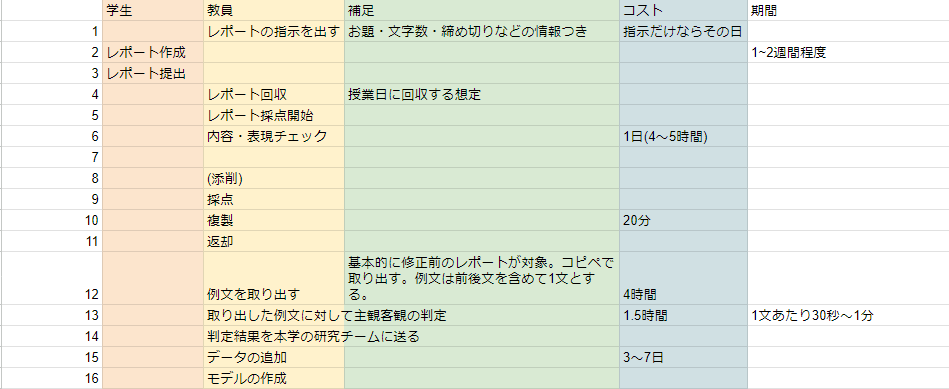
\includegraphics[width=150mm]{image/systemsimurate.png}
	\label{simurate}
\end{table}

以上の工程を整理し,専門的な工程を除けば,例文を取り出す工程が最もコストが高いと考え,本システムとは独立したグレーゾーン表現を含む文章を取り出すツールの構築をおこなった.本ツールは,Python,話しことばチェッカーでも使用されているMeCabを用いて作成しており,グレーゾーンを含む1文および,その前後1文ずつの計3文を抽出している.これは,グレーゾーンを含む文章の主観性・客観性の判定時の補足情報に用いるためである.

\begin{figure}[H]
	\centering
 	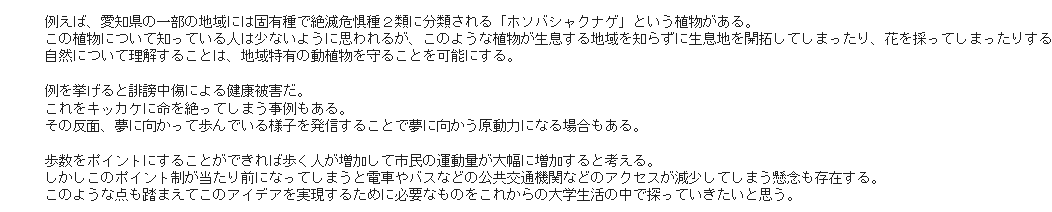
\includegraphics[width=150mm]{image/tool-grayfinder.png}
        \caption{ツールの実行結果}
	\label{grayfinder}
\end{figure}

本ツールにより,成分を取り出す工程の期間の削減が見込められるが,以降の主観性・客観性の判定は,専門家の知識や判断が重要となる.そこで,近年台頭しているLLMの活用を試みた.LLMは対話型の生成AIであり,文脈を読み取れる特性を持つことから,文章の主観性客観性の判断が可能であることが考えられる.グレーゾーンのラベル付けにLLMが活用できると仮定し,グレーゾーン「てしまう」を含む文章の主観客観の判定を通し,ラベル付け工程の代替となり得るかを調査した.